\section{Our solution}
To tacle this issue we will be subdividing the problem in to 5 different modules which include:

\begin{itemize}
\item[\textbullet] Random Process Generator
\item[\textbullet] Client module
\item[\textbullet] Bike module
\item[\textbullet] Central Scheduler
\item[\textbullet] Graphical Interface
\end{itemize}

Each part with their various specifications which are elaborated as follows

% --------------RPG-----------------------
\subsection{Random Process Generator(RPG)}
The RPG (Random Process Generator) serves as a crucial tool in simulating the behavior of real-world customers  and bikers within a ride command system.\\This RPG as stated above is used for customers and bike generation and is further explained as follows:

\subsubsection{Client-RPG}
The RPG (Random Process Generator) is a crucial tool designed to simulate the behavior of real-world customers within a ride command system. In parallel, it generates ride requests for bikes at random intervals, replicating the unpredictable patterns of user behavior in a live environment.\\\\Specifically designed for this context, the RPG generates ride requests for bikes and customers at random intervals, replicating the unpredictable patterns of human behavior in a live environment.

\subsubsection{Bike-RPG}
In parallel, another component of the system creates bikes to fulfill these randomly generated ride requests. This dual simulation process mimics the dynamics of the system's response in providing the necessary bikes to meet those requests within the framework.\\\\This approach allows developers to assess how well the system handles the variability in user demands, ensuring its ability to efficiently respond to spontaneous ride requests and allocate bikes accordingly. This thorough testing contributes to enhancing the overall reliability and effectiveness of the ride command system in meeting the dynamic needs of its users.
%-------------------------------------

% ------------Client-------------------
\subsection{Client module}
For this section, we have decided to use shared memory segments. The following provides an overview of how the client operates. 

On creation of a motorcycle the following steps are followed:
\begin{enumerate}
  \item \textbf{Information Generation}:by using four random values, the first determining its starting point, the second defining its final point and the third being its process id and the time waiting time limit, thus establishing all the necessary informations.
  \item \textbf{Shared Memory Segment Creation}: attaching to the client a shared memory in read-write mode.
  \item \textbf{Signal Transmission to Scheduler}: It then sends a signal to the scheduler informing the completion of the initial part execution.
  \item \textbf{Signal Awaiting}: It waits for the scheduler's signal which will continue until it reaches it's limit. If the time allocated is over happens, the process is then terminated and send a signal to the scheduler and is removed from the  client list.
  \item \textbf{Signals Reception}: It receives a signal from the the bike informing them that they have been carried and. At the end of the ride it receives a signal from the bike stating the end of the ride and gets terminated.
\item \textbf{Signals Emission}: It finally sends a signal from the the scheduler stating the end of the procedure.\\\\
\end{enumerate}

% -------------------------------------

% --------------Bike-------------------
\subsection{Bike module}
For this section as the one above, we have decided to use shared memory segments. The following provides an overview of how the motorcycle operates. 

On creation of a motorcycle the following steps are followed:
\begin{enumerate}
  \item \textbf{Route Creation}:by using two random values, the first determining its starting point and the second defining its "radius" thus establishing its itinerary.
  \item \textbf{Shared Memory Segment Creation}: attaching to the bike a shared memory in read-write mode.
  \item \textbf{Signal Transmission to Scheduler}: It then sends a signal to the scheduler informing the completion of the initial part execution.
  \item \textbf{Signal Awaiting}: It waits for the scheduler's signal which is reading the list clients stored in the shared memory segment and since we decided to implement the FIFO policy, it selects the first client in the list.
  \item \textbf{Signal Reception}: It receives a signal from the scheduler assigning it a client to serve.
  \item \textbf{Signal Transmission to Client}: It then sends a signal to the client informing them that they have been carried.
  \item \textbf{Waiting}: It then sends a signal to the scheduler indicating the transportation of a client. Which in our case is synonymous to going into the waiting state.
  \item \textbf{End signal}: It sends a signal to the client indicating to end of it's process.
  \item \textbf{Restart}: The procedure then restarts from the beginning.
\end{enumerate}

As such we will have completed the total transport of a client and managed potential deadlock situations.
% ---------------------------------------

%--------Central Scheduler---------------
\subsection{Central Scheduler}
When creating the central scheduler the following steps are followed:
\begin{enumerate}
  \item \textbf{Data initialization}:Here we start by creating two deques one for the clients and another one for the bikes which are present. And then arm the different signal handlers.
  \item \textbf{Listening Mode}: The Scheduler now listens to the various signals from bikes and the clients for a set time t.
  \item \textbf{Masking of signals}: After the said time, the signals sent as of now are not taken into consideration for the following scheduler operations
  \item \textbf{Saving Clients and Bikes information}: It saves the different clients into the deque saving it using the FIFO policy and same is done for the different bikes using the other deque.
  \item \textbf{Assigning Clients to Bikes}: Using the first fit protocole, the various clients are assigned to the available bikes and for this to happen, a signal is sent to the chosen bike and the chosen client is removed from client deque.
  \item \textbf{Restart}: The procedure then restarts from the listening period and the masked items are added to the appropriate deques.
\end{enumerate}

%-----------------------------------------

\newpage

%-----------User Interface-----------
\subsection{simulation:User Interface}
Using OpenGL, we now create the different representations for the clients represented by a \textcolor{blue}{blue} \textbf{circle}, the bikes represented by a \textcolor{green}{green} \textbf{square} and quarters differentiated by various colours and shapes.\\
Both bikes and clients only appear when they have been matched.


The following figure gives a brief summary of all what has been explicated above.
The numbered sections 0.a, 0.b, 0.c, 0.d, 2.a and 2.b which couldn't be further explained on the figure respectively represent the following:

\begin{enumerate}
  \item \textbf{Step 0.a}:This represents the information generation and the shared memory segment creation.
  \item \textbf{Step 0.b}: This represents the route and the shared memory segment creation.
  \item \textbf{Step 0.c}: This part is concerned with the data initialization and listening mode from the scheduler
  \item \textbf{Step 0.d}: This part is concerned with the initialization of the user interface
  \item \textbf{Step 2.a}: This part is concerned with the different saving of the different bikes and clients information.
  \item \textbf{Step 2.b}: This part is concerned with the the treatment of all the various signals by the user interface.
\end{enumerate}
%-----------------------------------------
\begin{center}
   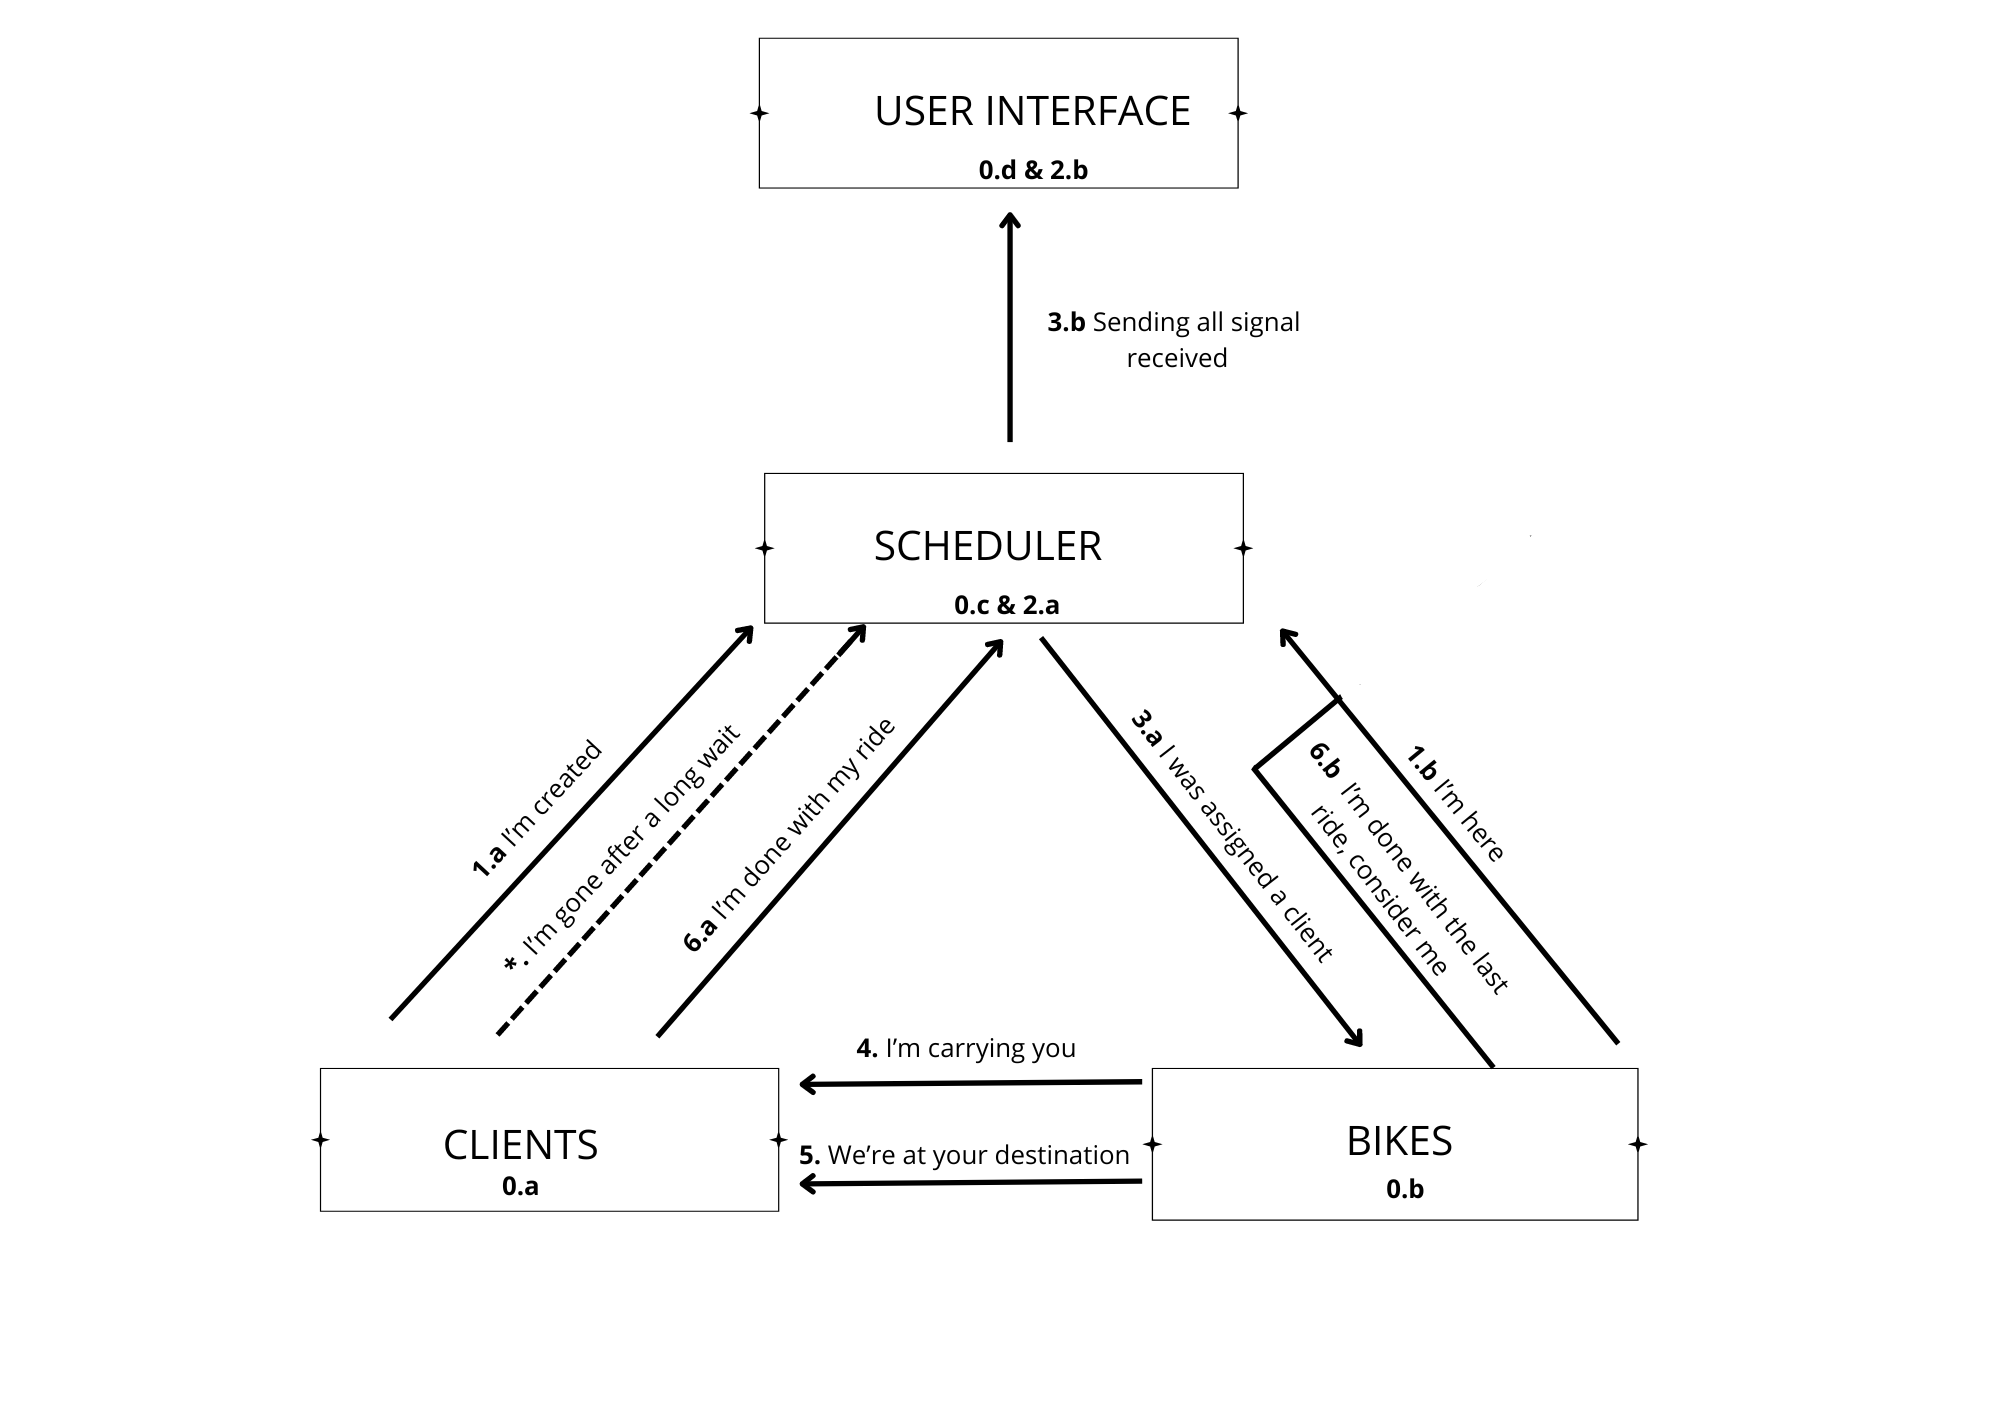
\includegraphics[width=1.0\linewidth]{Sections/Images/fro.png}
\end{center}
